\documentclass[12pt]{article}

\usepackage{amsmath}
\usepackage{geometry}
\usepackage{xcolor}
\usepackage{tikz}
\usetikzlibrary{arrows.meta, patterns}
\geometry{margin=1in}

\setlength{\parskip}{0.5em}

\begin{document}

\title{Circular Dynamics Examples}
\author{}
\date{}
\maketitle

\vspace{1em}

\section*{Example 1: The "Role" of Centripetal Force}
\textit{Corresponds to Notes Section 1.2: The "Role" Analogy}

\textbf{Problem:}
A $0.150 \, \text{kg}$ ball is attached to a string and swung in a horizontal circle on a frictionless table. The radius of the circle is $0.600 \, \text{m}$, and the ball moves at a constant speed of $4.00 \, \text{m/s}$. 
Identify the physical force acting as the centripetal force and calculate its magnitude.

\newpage

\section*{Example 2: Car on a Flat Curve}
\textit{Corresponds to Notes Section 2.1}
\textbf{Problem:}
A $1200 \, \text{kg}$ car is making a turn on a flat, unbanked road with a radius of curvature of $45.0 \, \text{m}$. The coefficient of static friction $\mu_s$ between the tires and the road is $0.650$. What is the maximum speed the car can travel without skidding?

\newpage

\section*{Example 3: The Conical Pendulum}
\textit{Corresponds to Notes Section 2.2}

\textbf{Problem:}
A $0.500 \, \text{kg}$ mass is attached to a string and swings in a horizontal circle. The string makes an angle of $30.0^\circ$ with the vertical. The radius of the circular path is $0.400 \, \text{m}$. Calculate the tension $T$ in the string and the speed $v$ of the mass.

\begin{figure}[h]
    \centering
    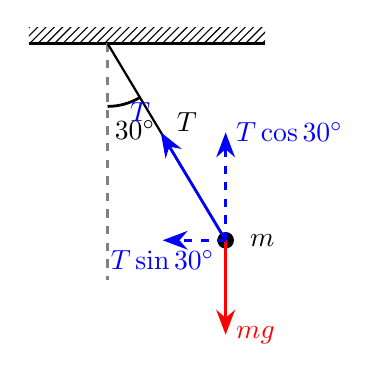
\begin{tikzpicture}[scale=1.0, line width=1pt]
        % Ceiling/Pole
        \draw[thick] (-1, 2) -- (2, 2);
        \fill[pattern=north east lines] (-1, 2) rectangle (2, 2.2);
        \draw[dashed, gray] (0,2) -- (0,-1);
        % Rope and Bob
        \coordinate (Bob) at (1.5, -0.5);
        \draw[thick] (0,2) -- (Bob) node[midway, above right] {$T$};
        \fill (Bob) circle (3pt) node[right=5pt] {$m$};
        % Angle
        \draw (0, 1.2) arc (270:301:0.8); 
        \node at (0.35, 0.9) {$30^\circ$};
        % FBD components
        \draw[-{Stealth[scale=1.2]}, red] (Bob) -- ++(0, -1.2) node[right] {$mg$};
        \draw[-{Stealth[scale=1.2]}, blue] (Bob) -- ++(121:1.6) node[above left] {$T$};
        \draw[dashed, blue, -{Stealth[scale=1.2]}] (Bob) -- ++(0, 1.37) node[right] {$T\cos 30^\circ$};
        \draw[dashed, blue, -{Stealth[scale=1.2]}] (Bob) -- ++(-0.8, 0) node[below] {$T\sin 30^\circ$};
    \end{tikzpicture}
\end{figure}

\newpage

\section*{Example 4: Vertical Circular Motion (Rollercoaster)}
\textit{Corresponds to Notes Section 3.1 \& 3.2}

\textbf{Problem:}
A rollercoaster cart (mass $m = 400 \, \text{kg}$ including passengers) is going through a vertical loop with a radius of $12.0 \, \text{m}$.
\begin{enumerate}
    \item[(a)] What is the critical (minimum) speed required at the \textbf{top} of the loop to prevent the cart from falling off?
    \item[(b)] If the cart goes through the \textbf{bottom} of the loop at $20.0 \, \text{m/s}$, what is the Normal force exerted by the track on the cart?
\end{enumerate}

\newpage

\section*{Example 5: Work and Energy in Circular Motion}
\textit{Corresponds to Notes Section 4}

\textbf{Problem:}
An artificial satellite of mass $1000 \, \text{kg}$ is in a perfectly circular orbit around the Earth. During one full orbit, how much work is done by the Earth's gravity on the satellite? Does the kinetic energy of the satellite change?

\vspace{8cm}

\end{document}
